\begin{center}
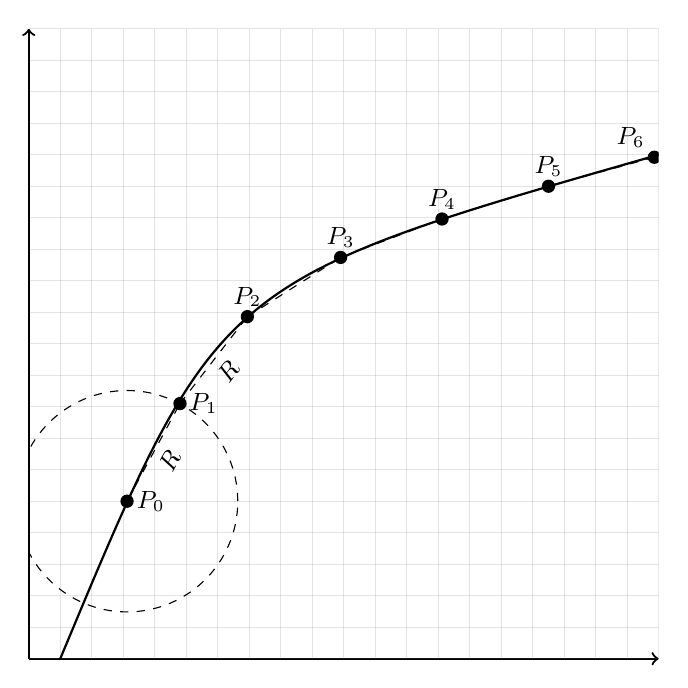
\begin{tikzpicture}
	[scale = 0.8,
	axis/.style={->, black, thick}]
	
	% Draw main axes
	\draw[axis] (0, 0) -- (10, 0);
	\draw[axis] (0, 0) -- (0, 10);
	
	\clip (0,0) rectangle (10, 10);
	
	% Draw grid
	\foreach \x in {0, 0.5, ..., 10.1}
		\foreach \y in {0, 0.5, ..., 10.1}
		{
			\draw[thin, gray, opacity=0.01] (\x, 0) -- (\x, 10);
			\draw[thin, gray, opacity=0.01] (0, \y) -- (10, \y);
		}
		
	% Draw path
	\draw[thick] (0.5, 0) .. controls (3, 6) .. (10, 8);
		
	% Draw first point
	\coordinate (P1) at (1.56, 2.5);
	\fill (P1) circle[radius=3pt] node[anchor=west]{\small $P_0$};
	\draw[dashed] (P1) circle[radius=50pt];

	% Draw second point
	\coordinate (P2) at (2.4, 4.05);
	\fill (P2) circle[radius=3pt] node[anchor=west]{\small $P_1$};
	
	% Draw third point
	\coordinate (P3) at (3.47, 5.43);
	\fill (P3) circle[radius=3pt] node[anchor=south]{\small $P_2$};
	
	% Draw fourth point
	\coordinate (P4) at (4.95, 6.37);
	\fill (P4) circle[radius=3pt] node[anchor=south]{\small $P_3$};
	
	% Draw fifth point
	\coordinate (P5) at (6.56, 6.98);
	\fill (P5) circle[radius=3pt] node[anchor=south]{\small $P_4$};
	
	% Draw fifth point
	\coordinate (P6) at (8.25, 7.5);
	\fill (P6) circle[radius=3pt] node[anchor=south]{\small $P_5$};
	
	% Draw seventh point
	\coordinate (P7) at (9.93, 7.96);
	\fill (P7) circle[radius=3pt] node[anchor=south east]{\small $P_6$};
	
	\draw[dashed] (P1) -- (P2) node[midway, below, sloped] {\small $R$};
	\draw[dashed] (P2) -- (P3) node[midway, below, sloped] {\small $R$};
	\draw[dashed] (P3) -- (P4) -- (P5) -- (P6) -- (P7);
	
\end{tikzpicture}
\end{center}